\section{Visualization}
\subsection{Geographic Map}
The first component of our visualization is the geographic map, whose goal is to show to the end customer the precise projected point (using longitude and latitude fields) where a particular battle occurred. In particular, we took an European continent picture with its respective countries boundaries information, and projected the real battles coordinates over it, in order to properly fit them to our figure. We represented each battle with a clickable circle, which color depends on the battle outcome. In order to known the battle details that has been selected, we provided also a small legend that summarize some useful information such as battle name, year, coordinates and outcome. Furthermore, is possible to select multiple battles via the brushing approach. In fact, when a number $n > 2$ of battles is selected, the legend will show that n battles has been selected and also the time period in which they have been occurred, hiding unselected battles. In this scenario, the other charts of the visualization will be properly updated. Conversely, also the geographic map will be updated when a particular time period is selected in the Line chart or a group of battles is selected in the Scatter plot. In the first case, the battles outside the selected time period will be hidden, whereas in the second scenario the selected battles will be highlighted with a black border.
\begin{figure}[h]
\centering
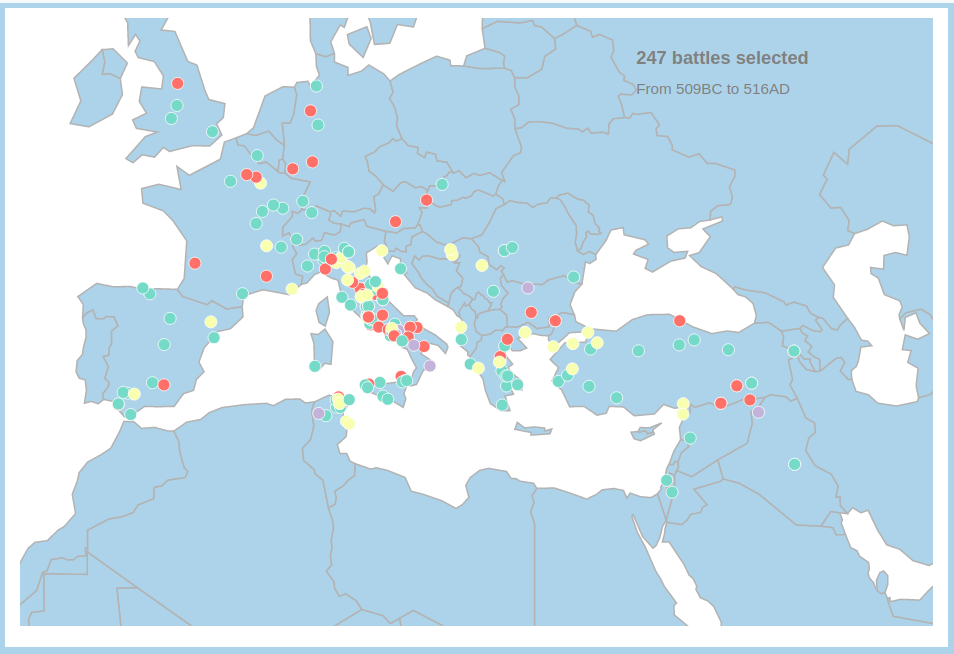
\includegraphics[scale=0.20]{./images/geographic_map.png}
\caption{Geographic map}
\end{figure}

\subsection{Line Chart}
The next component is the Line chart, which is responsible to communicate to the analyst the trends of won and lost battles in a given time period. We provided two analysis approaches : \textbf{by centuries} in order to analyze the previous trends from a general point of view in century form, the second one is \textbf{cumulative}, which allow us to perform a more specific analysis with respect to the previous one, taking into account the trends in year form. The Line chart has two axis : the x axis represents centuries or years, and the y axis represents the number of battles. The first interaction on this chart is reached through brushing plus zooming approach. In fact, selecting a specific time period via brushing, the zoom function will update the chart axis's ranges and data. To remove a selection the user just have to perform a double click. In this scenario, the selected data will update also the geographic map, stacked bar chart and scatter plot. In contrary, this chart will be updated only if any changes occurs in the geographic map.
\begin{figure}[h]
\centering
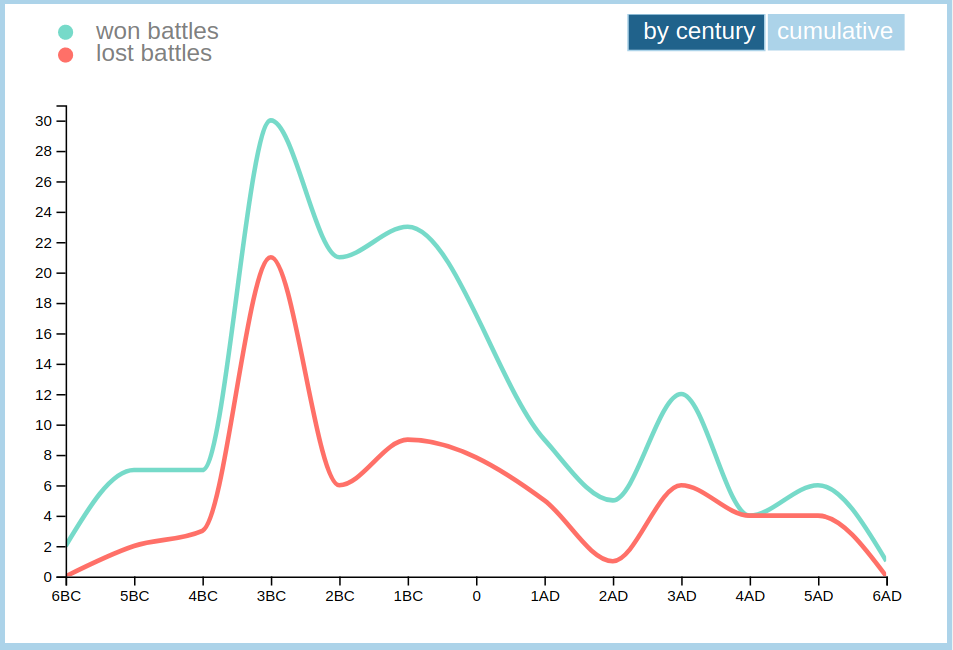
\includegraphics[scale=0.20]{./images/line_chart.png}
\caption{Line chart}
\end{figure}

\subsection{Stacked Bar Chart}
The stacked bar chart is another component of our visualization that offers a different type of analysis. It's constituted by two axis : the x axis represent two battle types \textbf{sacks} and \textbf{sieges}, the y axis represent the number of the battles. This analysis is based on won, lost and uncertain battles (as usual we reported a legend for reason of clarity). This chart is not able to update the other ones, but can be updated with a selection performed in the geographic map, in the line chart or over both of them. In case of doubts about the number of battles outcome with a particular type, we just have to move the mouse pointer over that layer, and will be shown a small label that contains the exact number.
\begin{figure}[h]
\centering
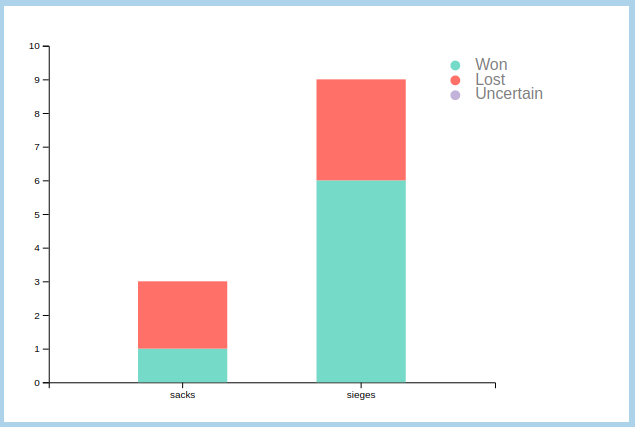
\includegraphics[scale=0.30]{./images/stacked_bar_chart.png}
\caption{Line chart}
\end{figure}

\subsection{Box Plot}
\todo[inline]{Describe the visualization component}
\missingfigure{Box Plot}

\subsection{Scatter Plot}

\begin{figure}[h]
\centering
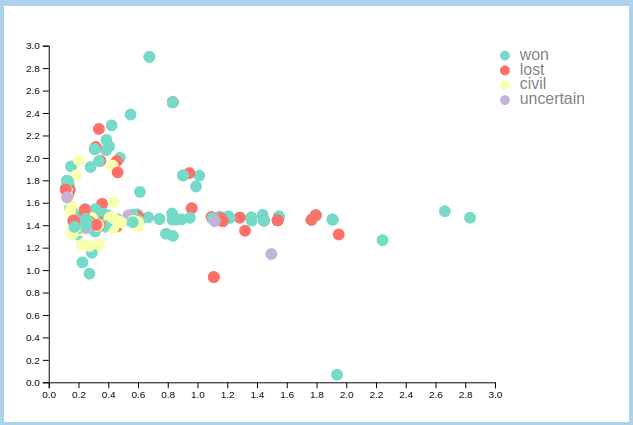
\includegraphics[scale=0.30]{./images/scatter_plot.png}
\caption{Line chart}
\end{figure}

\subsection{Filters - Header}
\todo[inline]{Describe the visualization component}
\missingfigure{Header filters}
